%\chapter{Desarrollo de propuesta de prototipo}\label{cap:capitulo4}

%---------------------------------------------------------------------------
\subsection{Creación de conjunto de datos de entrenamiento y adaptación de nanoGPT}\label{section:Creación de conjunto de datos con fuentes de internet} 
El conjunto de datos contiene recomendaciones y prácticas de seguridad clasificadas por categorías como amenazas, ataques y malware, figura \ref{figure:Conjunto de datos}. Esta clasificación permite que el modelo mejore clasifique mejor la entrada de texto dada.
\begin{figure}[H]
   \centering % figure is centered on the page
       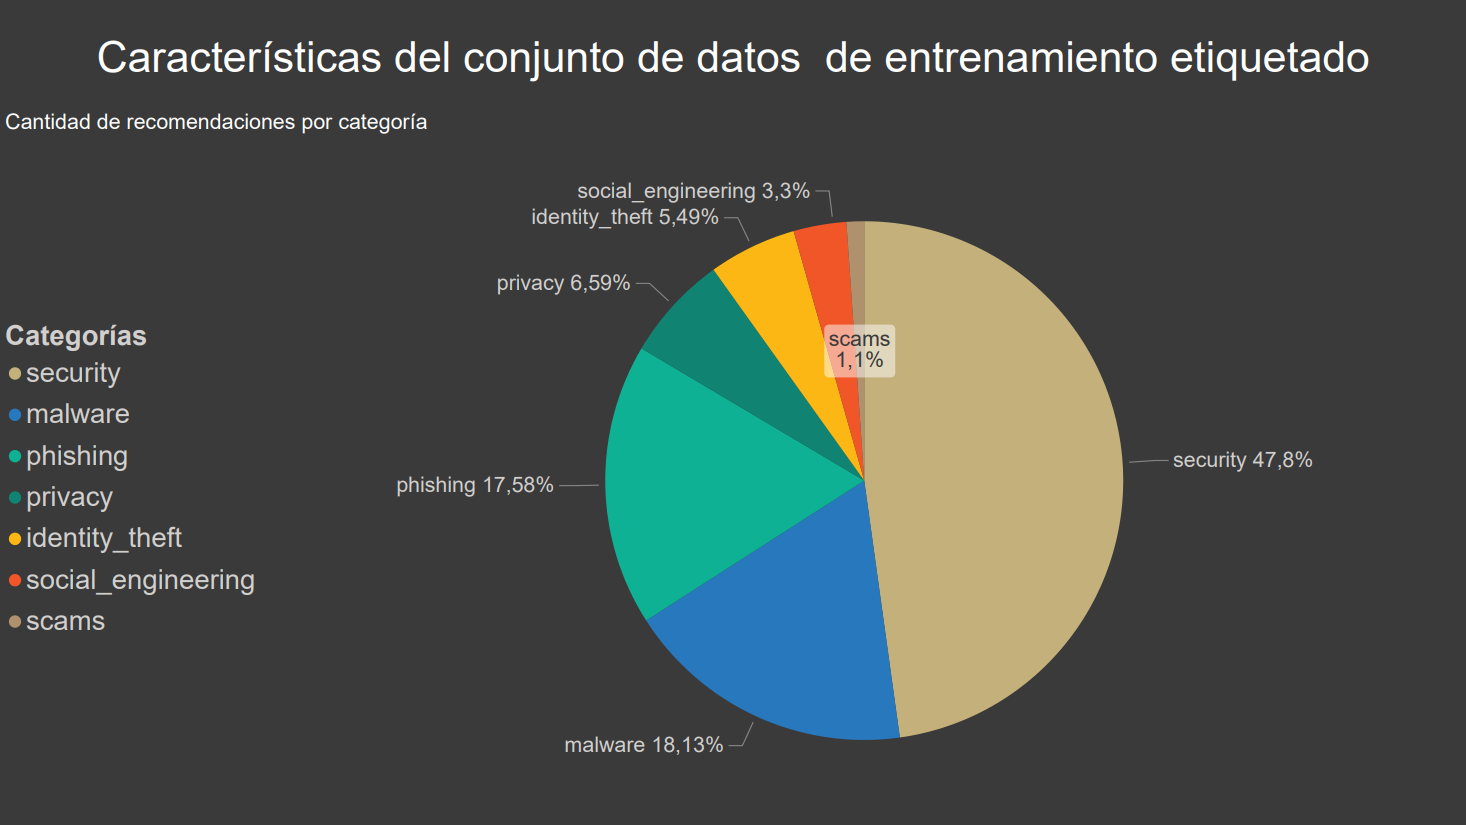
\includegraphics[width=0.7\linewidth]{./doc/Conjunto de datos etiquetado.png} 
   \caption{Características del conjunto de datos etiquetados \cite{}}
  \label{figure:Conjunto de datos}  % assign a unique label to each figure 
\end{figure}
%---Parrafo
El conjunto es se extrae desde el archivo CSV con el uso de la librería pandas a un dataframe. Figura \ref{figure:Extraxión de datos del csv}.\cite{Reiss2021}
\begin{figure}[H]
   \centering % figure is centered on the page
       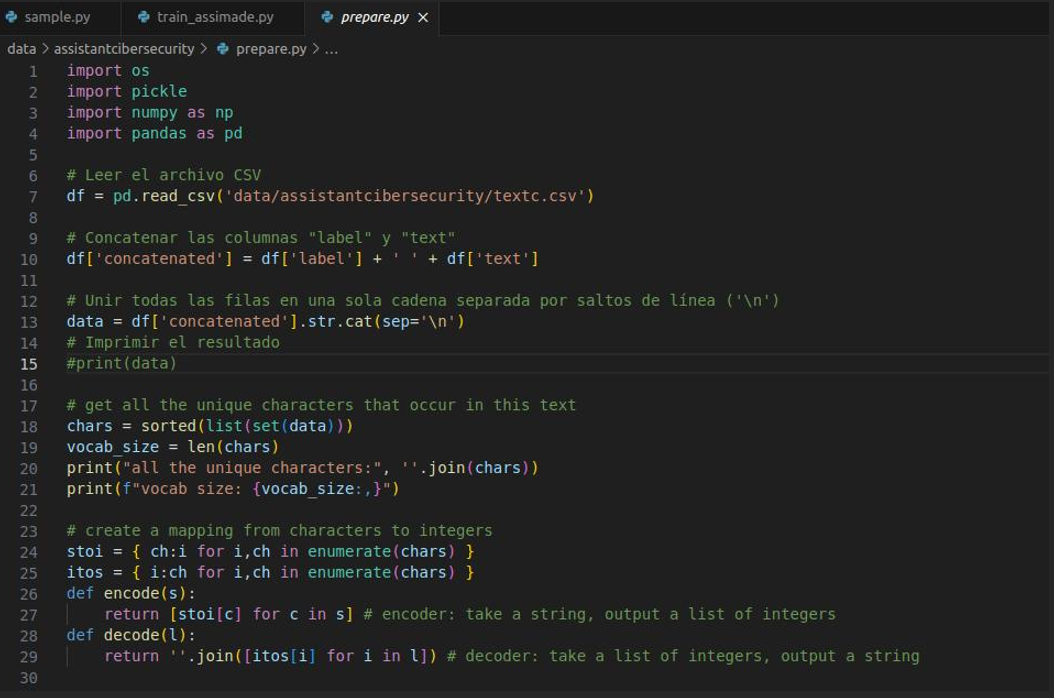
\includegraphics[width=0.8\linewidth]{./doc/02-cr.png} 
   \caption{Configuración para extraer el conjunto de datos en un dataframe y preparación de los datos.  \cite{}}
  \label{figure:Extraxión de datos del csv}  % assign a unique label to each figure 
\end{figure}
Para el entrenamiento con NanoGPT se crean las carpetas del conjunto de datos, se realiza el proceso de mapeo de caracteres a enteros también llamado vectorización para representar los datos de texto en secuencias de números. \cite{GenerGediz2020}
En la figura \ref{figure:Etapa de encoder}
\begin{figure}[H]
   \centering % figure is centered on the page
       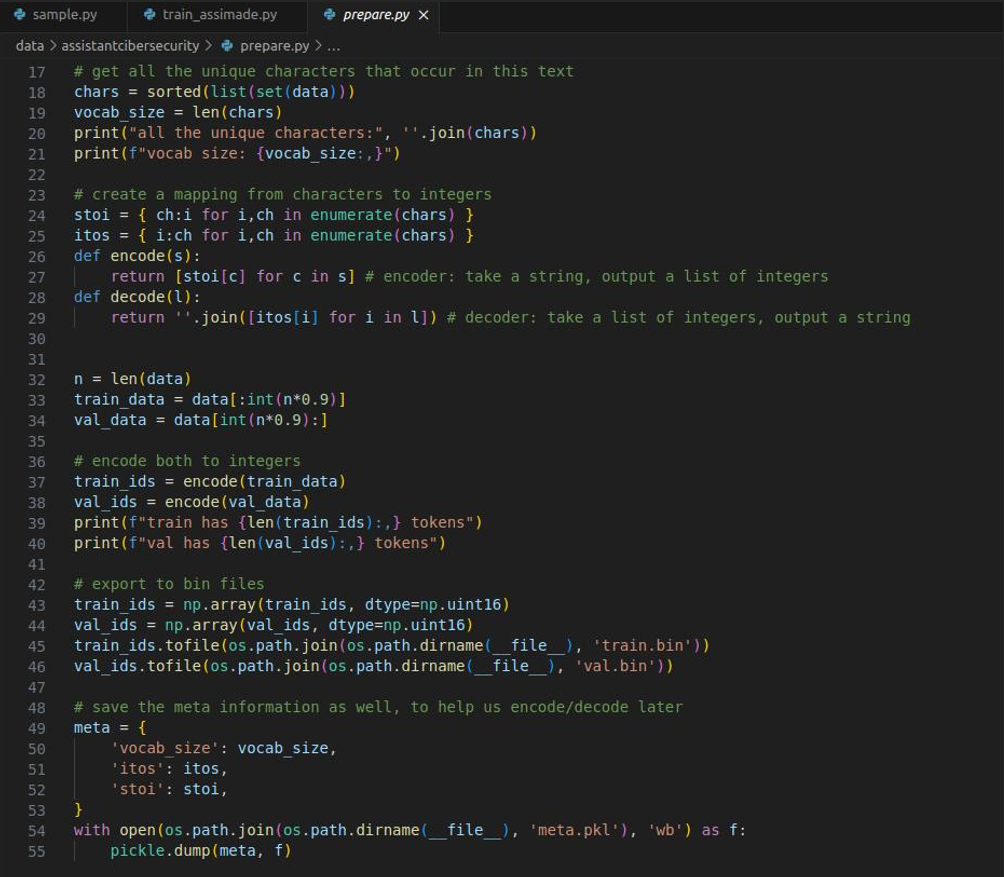
\includegraphics[width=0.8\linewidth]{./doc/03-cr.png} 
   \caption{procesamiento crea  ficheros de validación, entrenamiento y un meta modelo de apoyo.  \cite{}}
  \label{figure:Etapa de encoder}  % assign a unique label to each figure 
\end{figure}
%Parrafo-----
El procesamiento anterior crea ficheros de validación, entrenamiento y uno que contiene metadatos de los diccionarios para transformar de índices a palabras y viceversa para apoyo al proceso de condificación y decodificación.
\begin{figure}[H]
   \centering % figure is centered on the page
       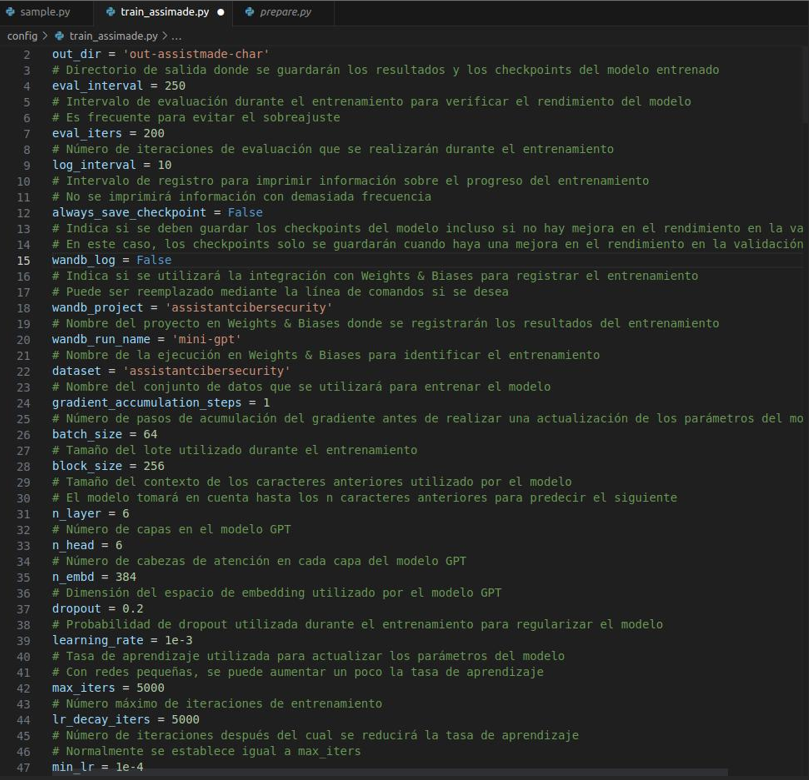
\includegraphics[width=0.8\linewidth]{./doc/04-cr.png} 
   \caption{Configuraciones y parámetros de entrenamiento que crea los directorios de salida para el modelo entrenado.  \cite{}}
  \label{figure:Configuraciónes de parámetros}  % assign a unique label to each figure 
\end{figure}
\clearpage
%---------------------------------------------------------------------------
\subsection{Configuración de los parámetros del código y entrenamiento}\label{section:Configuración y entrenamiento} 
Posteriormente se configuran dos modelos de prueba con variaciones de parámetros basados intervalos de entrenamiento, tamaños de bloque de texto procesado, cantidad de lotes en paralelo, ciclos de entrenamiento. 
Estas se realizado sobre la CPU, por lo que las configuraciones están centradas en entrenamientos de bajo rendimiento, el propósito es verificar configuraciones que permitan al modelo clasificar la entrada de texto y el conjunto entrenado.
%-------------------------------------------------------------------------------
%------------------------------------------------------------------------------
\subsubsection{Configuración parámetros}\label{section:Configuración de los parámetros del código} 
En la figura \ref{figure:Configuraciones modelo entrenamiento 2} se asignan a los parámetros:
\begin{enumerate}
	\item Evaluación cada 50 iteraciones con subconjunto creado en el procesamiento, esto permite que el modelo se ajuste de ser necesario. también se establece un tamaño de bloque que permite procesar una secuencia de entrada , el tamaño de lote en 32 para establecer ejemplos que se procesan de forma paralela.
	\item Secuencias de texto de tamaño en bloques de 128 que se procesan de manera secuencial, el lote de 32 para permitir cargas en paralelo.
	\item Configuración de las capas de la red en 4 capas las cuales tienen cada una cuatro capas de atención.
	\item Los vectores de incrustación en 256 para representar las palabras numéricamente vectores.
	\item Para la red neuronal se utilizan 4 capas de profundidad y 4 capas de atención que dan al modelo capacidad para capturar diferentes partes del texto que pueden ser relevantes para la clasificación. 
	\item Para establecer el tamaño de los vectores se establece en 256 para vectorizar una mayor cantidad de palabras en la oración  que permitan identificar representaciones significativas.
	\item Por ultimo el parámetro para establecer las iteraciones de entrenamiento se establecen en 3000. 
\end{enumerate} 
\begin{figure}[H]
   \centering % figure is centered on the page
       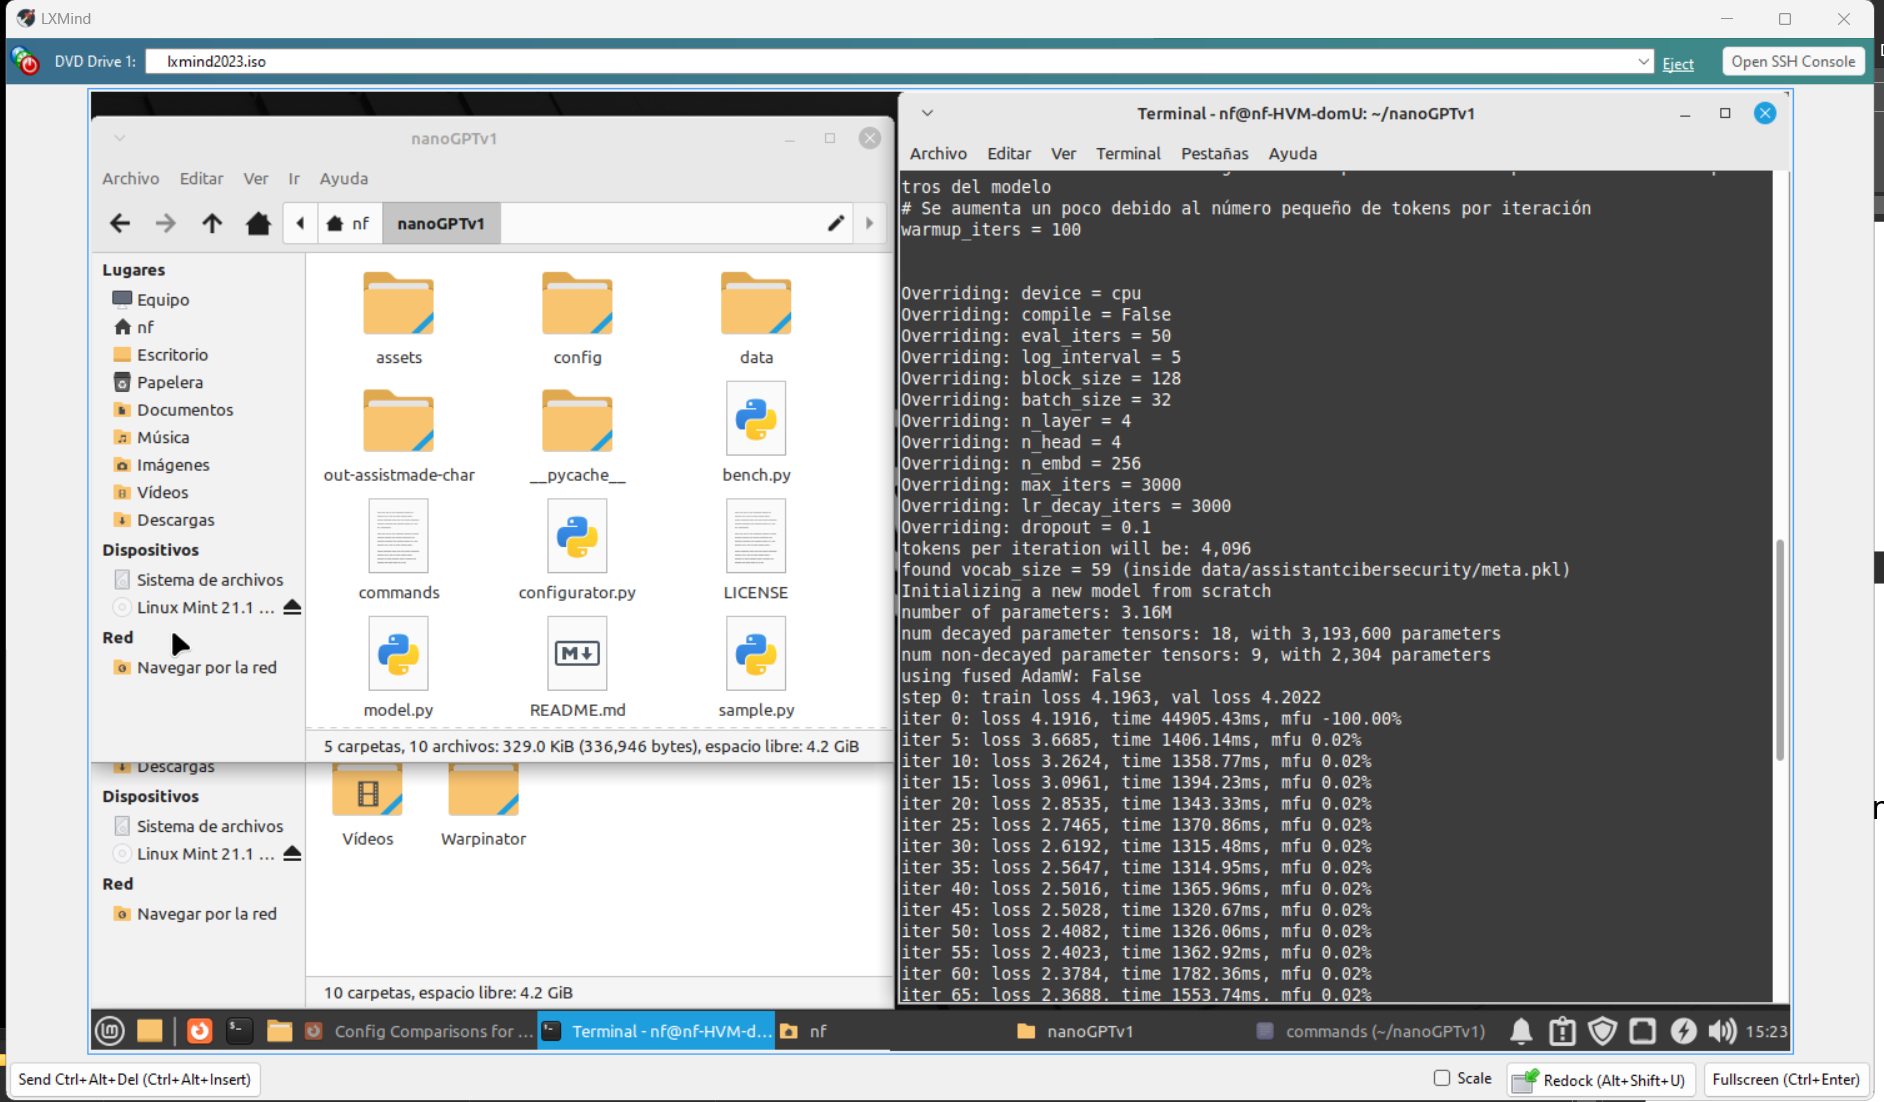
\includegraphics[width=0.65\linewidth]{./doc/Proceso de entrenamiento en XCP-ng.png} 
   \caption{Configuraciones de entrenamiento de modelo  \cite{}}
  \label{figure:Configuraciones modelo entrenamiento 2}  % assign a unique label to each figure 
\end{figure}
\begin{figure}[H]
   \centering % figure is centered on the page
       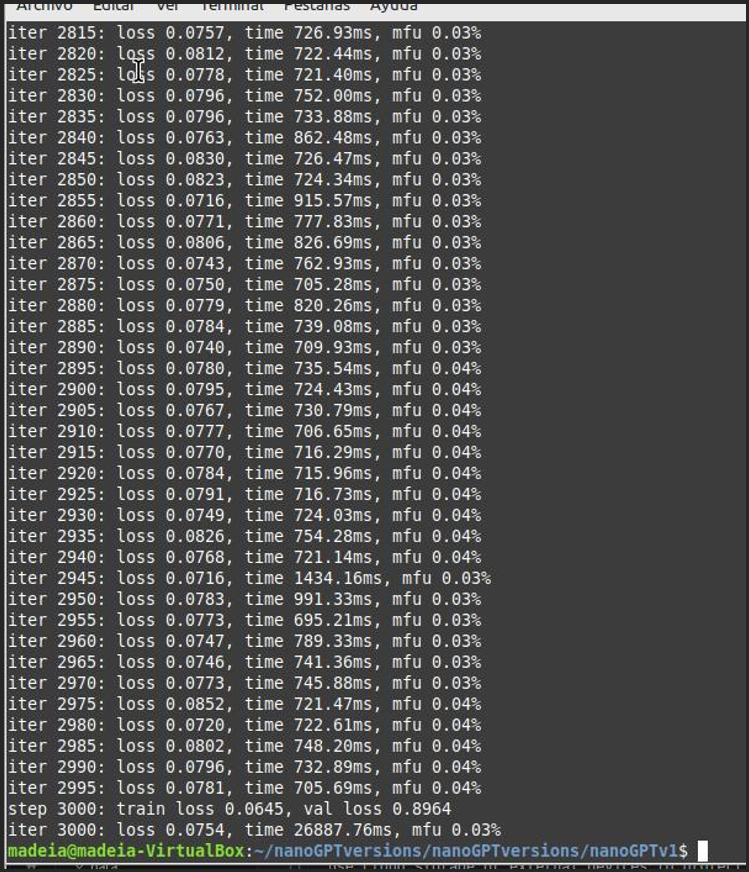
\includegraphics[width=0.65\linewidth]{./rp/06-cp.png} 
   \caption{Proceso de entrenamiento de modelo\cite{}}
  \label{figure:Proceso de entrenamiento del modelo}  % assign a unique label to each figure 
\end{figure}
%----------------------------------------------------------------------------
\clearpage
\subsection{Validación del modelo Configuración}\label{section:Validación de prompt}
\subsubsection{ Prueba 1}\label{section:Validación del prototipo}
    \begin{itemize}
        \item   Top-k = 100
        \item   Temperatura = 1.2
        \item   Ma-new-tokens = 500
        \item    Prompt = python3 sample.py --out-dir=out-assistmade-char --device=cpu --start=" phising protection tips"
    
\begin{figure}[H]
   \centering % figure is centered on the page
       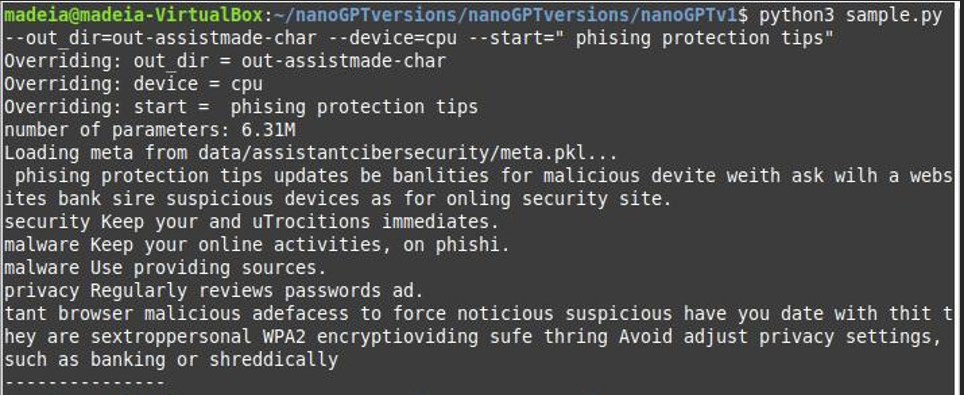
\includegraphics[width=0.65\linewidth]{./rp/16-cp.png} 
   \caption{Resultados de la Prueba 1\cite{}}
  \label{figure:Prueba1}  % assign a unique label to each figure 
\end{figure}
        \item   Prompt = python3 sample.py --out-dir=out-assistmade-char --device=cpu --start="safe internet browsing "
\begin{figure}[H]
   \centering % figure is centered on the page
       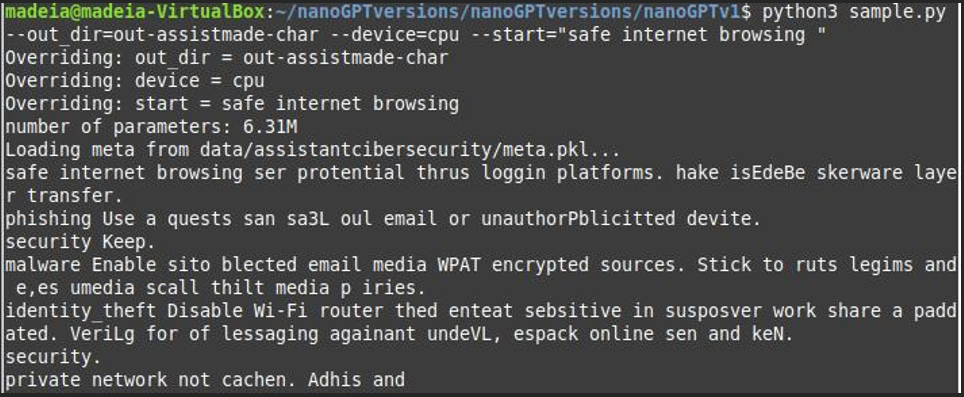
\includegraphics[width=0.65\linewidth]{./rp/17-cp.png} 
   \caption{Resultados de la Prueba 2\cite{}}
  \label{figure:Prueba2}  % assign a unique label to each figure 
\end{figure}
        \item   Prompt = python3 sample.py –out-dir=out-assistmade-char --device=cpu --start="computer security tips"
\begin{figure}[H]
   \centering % figure is centered on the page
       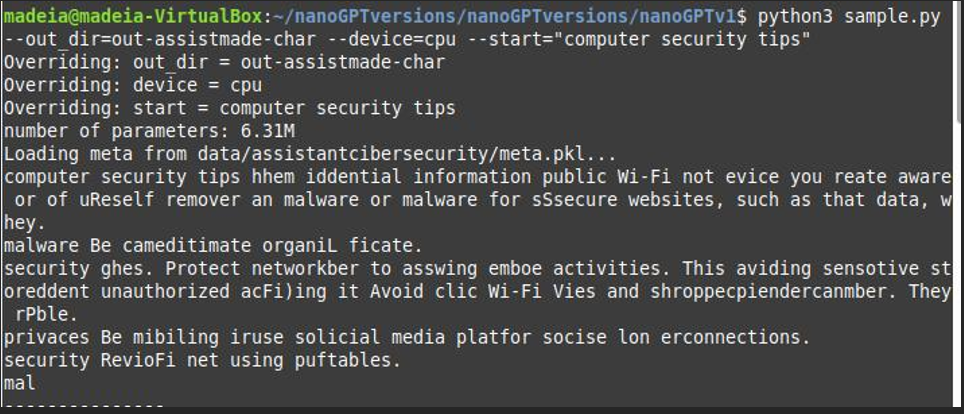
\includegraphics[width=0.65\linewidth]{./rp/18-cp.png} 
   \caption{Resultados de la Prueba 3\cite{}}
  \label{figure:Resultado prueba 3}  % assign a unique label to each figure 
\end{figure}
        \item   Prompt = python3 sample.py --out-dir=out-assistmade-char --device=cpu --start="prevent identity theft"
\begin{figure}[H]
   \centering % figure is centered on the page
       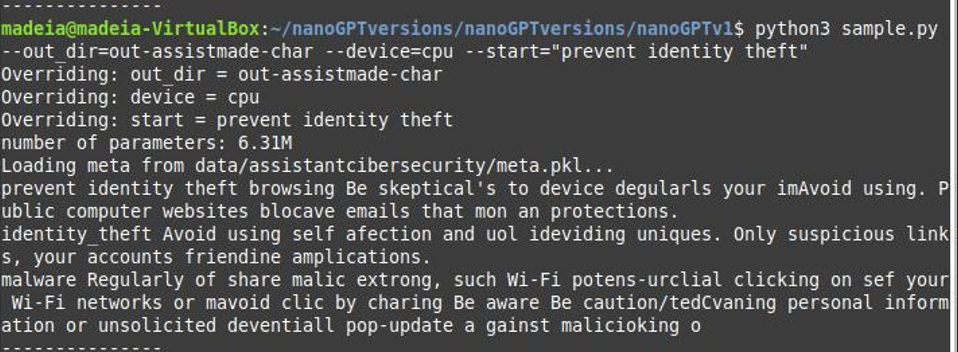
\includegraphics[width=0.65\linewidth]{./rp/19-cp.png} 
   \caption{Resultados de la Prueba 4\cite{}}
  \label{figure:Resultado prueba 4}  % assign a unique label to each figure 
\end{figure}
\end{itemize}
%-----------------------------------------------------------------------------   
\subsection{Validación del modelo Configuración 2}\label{section:Validación Modelo 2}
\subsubsection{ Prueba 1}\label{section:Prueba 1 config 2}
    \begin{itemize}
        \item   Top-k = 1
        \item   Temperatura = 10
        \item   Ma-new-tokens = 500
        \item    Prompt = python3 sample.py --out-dir=out-assistmade-char --device=cpu --start=" phising protection tips"
    \end{itemize}
\begin{figure}[H]
   \centering % figure is centered on the page
       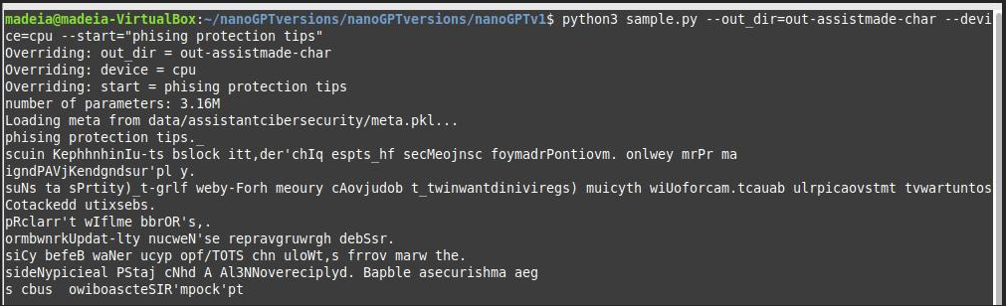
\includegraphics[width=0.65\linewidth]{./rp/07-cp.png} 
   \caption{Resultados de la Prueba 1\cite{}}
  \label{figure:Result prueba 1 mol 2}  % assign a unique label to each figure 
\end{figure}
\subsubsection{ Prueba 2}\label{section:Prueba2}
    \begin{itemize}
        \item   Top-k = 0.8
        \item   Temperatura = 10
        \item   Ma-new-tokens = 500
        \item   Prompt = python3 sample.py --out-dir=out-assistmade-char --device=cpu --start="safe internet browsing"
    \end{itemize}
\begin{figure}[H]
   \centering % figure is centered on the page
       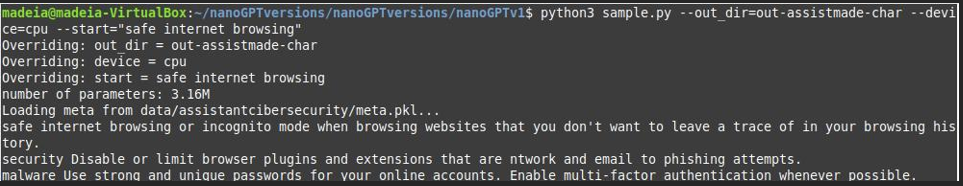
\includegraphics[width=0.65\linewidth]{./rp/08-cp.png} 
   \caption{Resultados de la Prueba 2\cite{}}
  \label{figure:Result prueb 2 mol 2}  % assign a unique label to each figure 
\end{figure}
\subsubsection{ Prueba 3}\label{section:Prueba 3 mol 2}
    \begin{itemize}
        \item   Top-k = 100
        \item   Temperatura = 1.2
        \item   Ma-new-tokens = 500
            \item   Prompt = python3 sample.py --out-dir=out-assistmade-char --device=cpu --start=" phising protection tips"
            \begin{figure}[H]
              \centering % figure is centered on the page
                  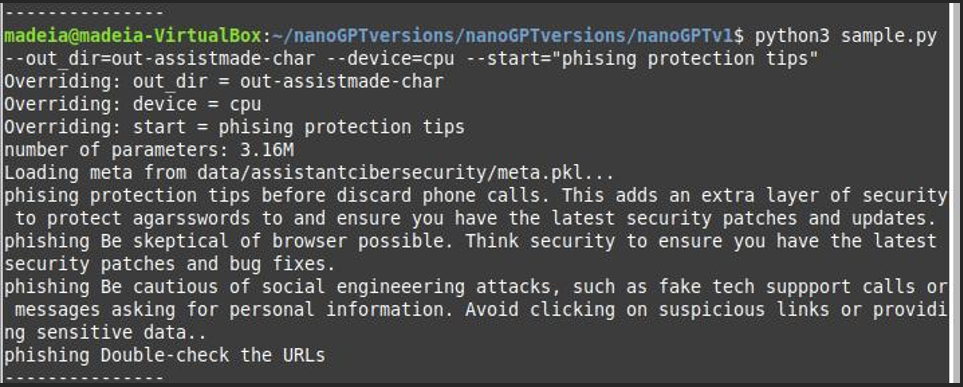
\includegraphics[width=0.65\linewidth]{./rp/09-cp.png} 
              \caption{Resultados de la Prueba 3.1\cite{}}
            \label{figure:Result Prueba 3 mod 2}  % assign a unique label to each figure 
            \end{figure}
            \item   Prompt = python3 sample.py --out-dir=out-assistmade-char --device=cpu --start="safe internet browsing"
            \item   Prompt = python3 sample.py --out-dir=out-assistmade-char --device=cpu --start="computer security tips"
            \begin{figure}[H]
              \centering % figure is centered on the page
                  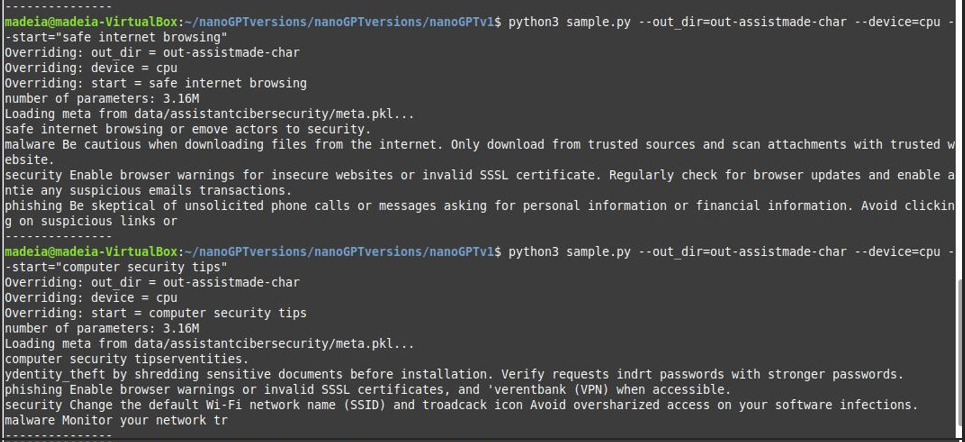
\includegraphics[width=0.65\linewidth]{./rp/10-cp.png} 
              \caption{Resultados de la Prueba 3.2 y 3.3\cite{}}
            \label{figure:Resultado 3.2}  % assign a unique label to each figure 
            \end{figure}
            \item   Prompt = python3 sample.py --out-dir=out-assistmade-char --device=cpu --start="computer security tips"
            \begin{figure}[H]
              \centering % figure is centered on the page
                  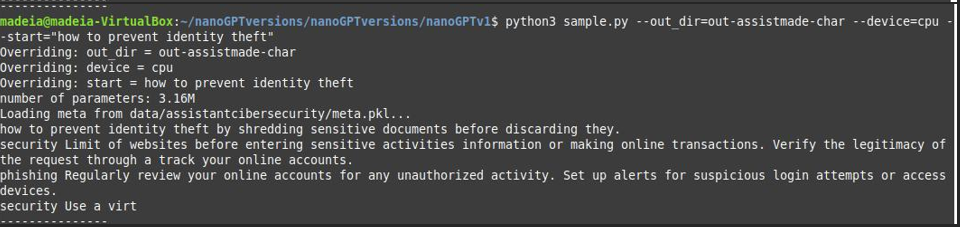
\includegraphics[width=0.65\linewidth]{./rp/11-cp.png} 
              \caption{Resultados de la Prueba 3.4\cite{}}
            \label{figure:Resultado 3.4}  % assign a unique label to each figure 
            \end{figure}
    \end{itemize}
\subsubsection{ Prueba 4}\label{section:Adaptación de modelo nanoGPT}
    \begin{itemize}
        \item   Top-k = 100
        \item   Temperatura = 1.1
        \item   Ma-new-tokens = 500
            \item   Prompt = python3 sample.py --out-dir=out-assistmade-char --device=cpu --start=" phising protection tips"
            \begin{figure}[H]
              \centering % figure is centered on the page
                  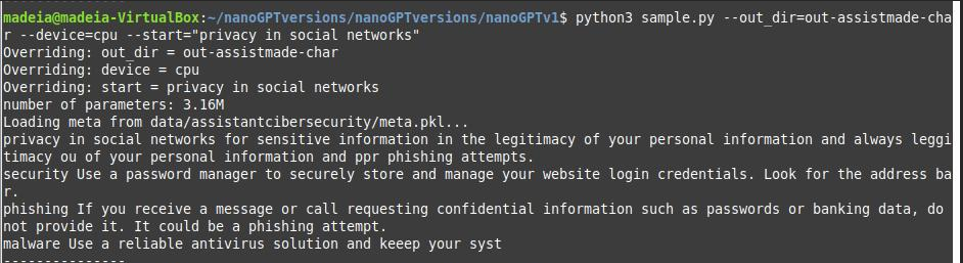
\includegraphics[width=0.65\linewidth]{./rp/12-cp.png} 
              \caption{Resultados de la Prueba 4.1\cite{}}
            \label{figure:Resultado 4 1}  % assign a unique label to each figure 
            \end{figure}
            \item   Prompt = python3 sample.py --out-dir=out-assistmade-char --device=cpu --start="computer security tips"
            \begin{figure}[H]
              \centering % figure is centered on the page
                  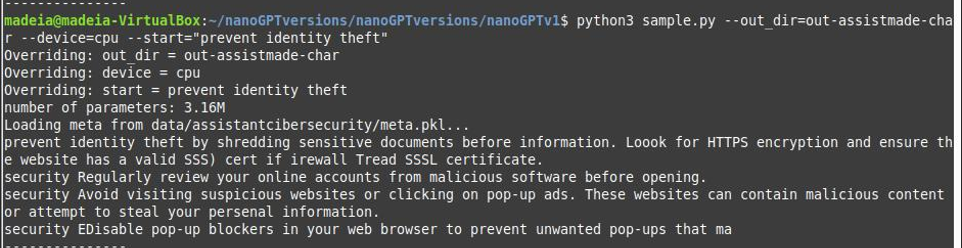
\includegraphics[width=0.65\linewidth]{./rp/13-cp.png} 
              \caption{Resultados de la Prueba 4.2\cite{}}
            \label{figure:Resultado prueba 4 2}  % assign a unique label to each figure 
            \end{figure}
            \item   Prompt = python3 sample.py --out-dir=out-assistmade-char --device=cpu --start="computer security tips"
            \begin{figure}[H]
              \centering % figure is centered on the page
                  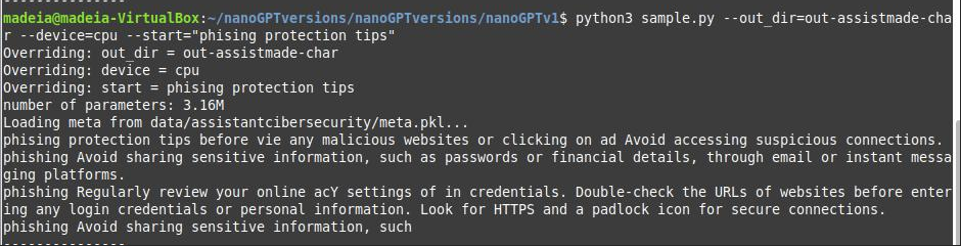
\includegraphics[width=0.65\linewidth]{./rp/14-cp.png} 
              \caption{Resultados de la Prueba 4.3\cite{}}
            \label{figure:Result prueba 4}  % assign a unique label to each figure 
            \end{figure}
    \end{itemize}
%---------------------------------------------------------------------------
%------------------------------------------------------------------------------

